\chapter{Data Set}
\label{Dataset}

\section{Overview}

In success of any software system that is based on deep neural networks, two main factors play a crucial role: network architecture and training data set. Although, a good network design is necessary for getting acceptable results; without an appropriate data set, training the network and getting any result is not possible. In fact, not only the quality of data set matters, but also as \citeauthor*{data} \cite{data} show, the performance of deep neural networks in vision tasks increases logarithmically based on volume of training data. 

For the task of surface normal estimation from RGB images of indoor scenes, a data set containing the RGB images and the corresponding surface normal maps is needed. As mentioned in related work section (page \pageref{sec:relatedwork}), it is possible to indirectly calculate the needed surface normal maps by using the depth map of the images. Therefore, to acquire such data set, a collection of images and their corresponding depth maps should be obtained; either by directly taking various pictures of indoor scenes or by using publicly available RGB-Depth data sets. 

Capturing new images is not only time consuming, but also makes it difficult to compare the results of the experiments with previously published results. Therefore, in this project, a publicly available RGB-D data set (NYU Depth V.2 \cite{silberman}) is used. All related work discussed in section \ref{sec:relatedwork}, use this data set for training their models. Also, to explore the effect of using a higher quality data set on improving network performance, a more recently released data set (SUN RGB-D \cite{sun}) is used in this project. 

There are several methods for computing the surface normal maps based on the depth map of the scene. For consistency with past research in this field and producing comparable results, this project used surface normal maps computed by using two more popular methods of \citeauthor*{ladicky} \cite{ladicky} and \citeauthor*{silberman} \cite{silberman}. These methods and the aforementioned data sets are discussed in next sections. 

\section{Publicly Available RGB-D Data Sets }

There are many existing RGB-D data sets available; but, only a few of them are suitable for the purpose of this project. For example, some data sets (such as \cite{objectdataset} and \cite{bigbird}) use a turntable for capturing the image of objects, instead of using real-world scenes. Even in data sets that use real-world indoor scenes, some of them (such as Berkeley 3-D Object Dataset \cite{b3do}) contain unrealistic scene layouts (e.g. snapshot of a computer mouse on the floor) or have a small size. In the following sections, two of the data sets that are more suited for use in this project are briefly introduced.

\subsection{NYU Depth V.2}

This data set has been the most popular data set for the task of surface normal estimation of indoor scenes. It is comprised of 1,449 pairs of aligned RGB and depth images, gathered from a wide range of commercial and residential buildings in three different US cities. These images are extracted from short video sequences captured by Microsoft Kinect version 1, from 464 indoor scenes across 26 scene classes. 

The data set has three components: the raw data (rgb, depth and accelerometer) as provided by the Kinect, preprocessed RGB and depth images, and a toolbox for data manipulation. In preprocessed part of the data set, in addition to the projected depth maps, a set of preprocessed depth maps whose missing values have been filled in (using the colourisation scheme of \citeauthor*{colorization} \cite{colorization}) is also included. This data set also provides meta-data about each image; which is irrelevant to this project (such as dense per-pixel labeling for each image). Figure \ref{fig:nyu} illustrates a few samples of this data set. 

\begin{figure}
    \centering
    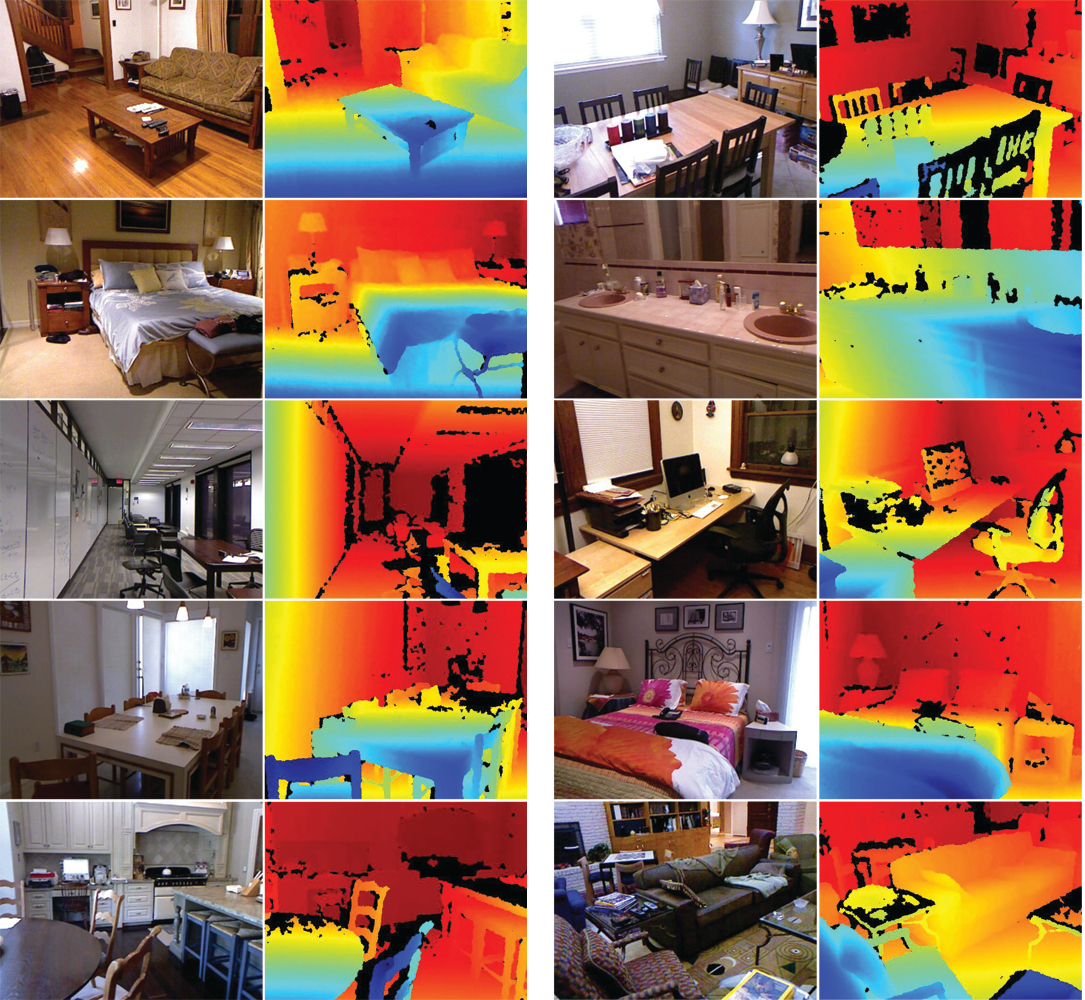
\includegraphics{NYU}
    \caption{NYU Depth V.2 data set, samples of the RGB images and the corresponding depth maps (missing data is coloured in black)\cite{silberman}}
    \label{fig:nyu}
\end{figure}

\citeauthor*{silberman} also suggest a train/test split for the samples of the data set. In this project, this split was used for selecting the samples for training and evaluation processes. The preprocessed samples and the toolbox are provided in format of MathWorks MATLAB files. 

\subsection{SUN RGB-D}

Princeton SUN RGB-D data set \cite{sun}, is a super-set of the NYU Depth V.2 \cite{silberman} data set. To construct this data set, \citeauthor*{sun} \cite{sun} capture 3,784 images using Microsoft Kinect v2 and 1,159 images using Intel RealSense sensors. They also include the 1,449 images from the NYU Depth V.2 data set and manually select 554 realistic scene images from the Berkeley B3DO Dataset \cite{b3do}. Finally, by including the manually selected 3,389 distinguished frames from the SUN3D \cite{sun3d} videos captured by Asus Xtion sensor, the total number of images in this data set reaches 10,335.

These RGB-D images are extracted from short videos captured from indoor scenes (such as universities, houses, and furniture stores) in North America and Asia. Like NYU Depth V.2, the raw depth maps captured by the depth sensors in this data set is not perfect; due to measurement noise, reflection of surfaces like mirrors, and occlusion boundaries. 

Also, the resolution of RGB images and the quality of raw depth maps captured by different sensors is not equal. Intel RealSense outputs noisier depth maps with more missing values, while Asus Xtion and Kinect v.1's depth maps have observable quantisation effects. Kinect v.2 captures depth maps with more details, but it is more sensitive to reflection and dark colours. Thus, to improve these depth maps, \citeauthor*{sun} propose an algorithm that uses depth data captured during multiple frames of the video, to obtain a single refined depth map for each image (Figure \ref{fig:sensors}). 

\begin{figure}
    \centering
    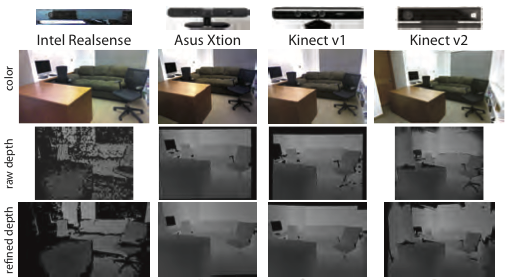
\includegraphics[width=\textwidth]{Sensors}
    \caption{Comparison of the four RGB-D sensors and the refinements in depth maps achieved by using the algorithm of \citeauthor*{sun} \cite[p.~2]{sun}}
    \label{fig:sensors}
\end{figure}

Alongside this data set, a toolbox (MathWorks MATLAB files) for loading and visualisation of data is also provided. The RGB images and depth maps are presented as PNG files.    

\section{Surface Normal Maps} \label{sec:surfnormmap}

As mentioned earlier, several different methods are used for computing the surface normal maps from depth data. In all related work discussed in chapter \ref{Background}, the published results are evaluated based on the surface normal maps computed by \citeauthor*{ladicky} \cite{ladicky} on the testing data set. For training the network, the raw data from the training data set is used. Because \citeauthor*{ladicky} have not published the surface normal maps for the raw data of the NYU Depth V.2 data set \cite{silberman}, the method of \citeauthor*{silberman} \cite{silberman} is used for computing these normal maps. \citeauthor*{dharmasiri} \cite{dharmasiri} also additionally evaluated their result based on the surface normal maps computed by the method of \citeauthor*{spek} \cite{spek}. 

\pagebreak

In this project, the method of \citeauthor*{silberman} \cite{silberman} was used for computing the surface normal maps in SUN RGB-D data set \cite{sun}. To get comparable results, surface normal maps provided by \citeauthor*{ladicky} \cite{ladicky} were used in evaluating the output of the networks.

In method used by \citeauthor*{silberman} \cite{silberman}, first by using the intrinsic parameters of the camera, the depth points are projected from image plane to the 3D world coordinates. Then, for the neighbouring sets of points in the 3D point cloud that their distance is not too large, a least-square plane is fitted. The normal vectors of these planes are the computed surface normals corresponding to the depth map points.  

On the other hand, \citeauthor*{ladicky} \cite{ladicky} first apply a denoising technique (based on the second order Total Generalized Variation (TGV) \cite{tgv}) on depth data. Then, normals are computed on the 3D point cloud for each point in a local 3D spatial neighbourhood. Finally, to estimate the point-wise normals, a least squares regression kernel in a RANSAC scheme is utilised in order to preserve surface edges \cite[p.~10]{ladicky}. 

The difference between these methods is due primarily to the fact that \citeauthor*{ladicky} \cite{ladicky} uses a more aggressive smoothing which results in flatter areas, while \citeauthor*{silberman} \cite{silberman} produces noisier results but with more details present \cite[p.~5]{eigen}. Figure \ref{fig:normalmethods} illustrates the difference in output of these methods.

\begin{figure}[h]
    \centering
    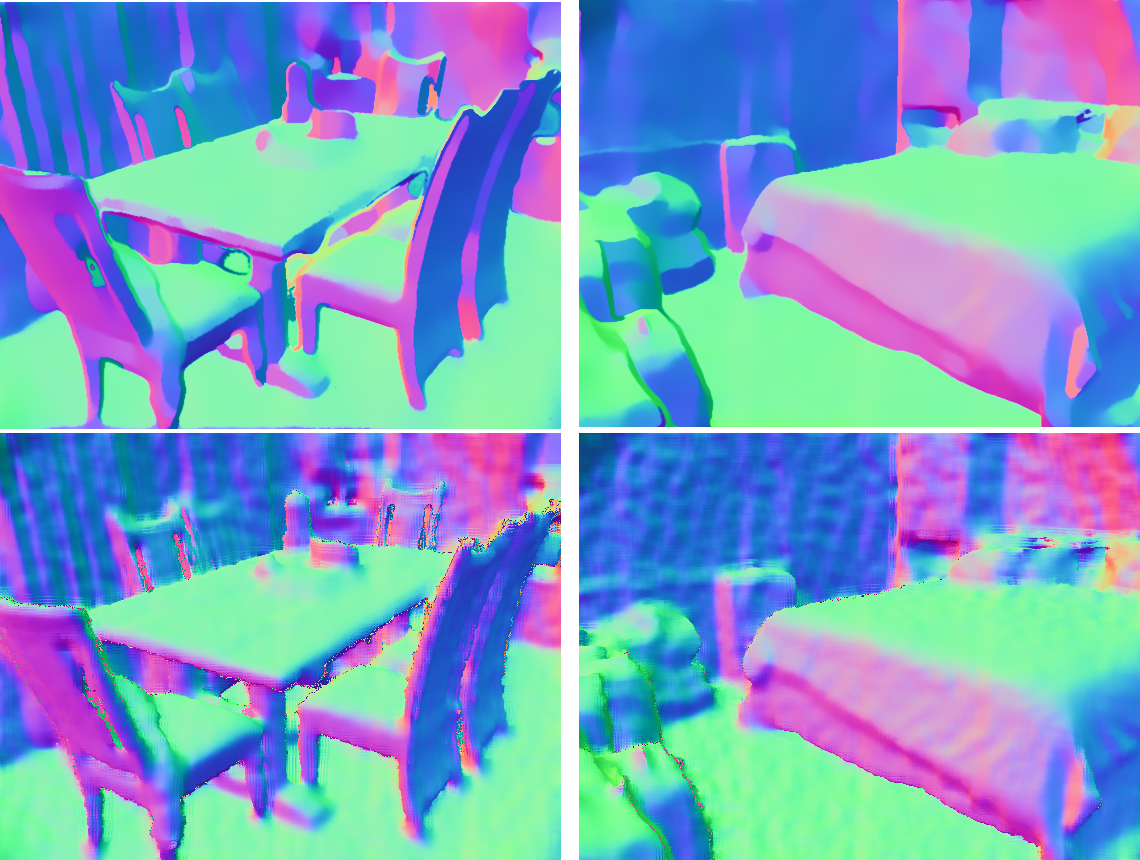
\includegraphics[width=\textwidth]{NormalMethods}
    \caption{Comparison of normal maps computed by different methods \\
    Top: based on \citeauthor*{ladicky} \cite{ladicky} , Bottom: based on \citeauthor*{silberman} \cite{silberman}  }
    \label{fig:normalmethods}
\end{figure}

\pagebreak

To reduce the noise presented in the output of \citeauthor*{silberman}'s method \cite{silberman}, inspired by the work of \citeauthor*{wang}, a denoising technique (total variation regularised least-squares deconvolution \cite{chan}) was applied on the computed normal maps in this project. Figure \ref{fig:denoisedsilberman} illustrates the results obtained by applying this method.

\begin{figure}
    \centering
    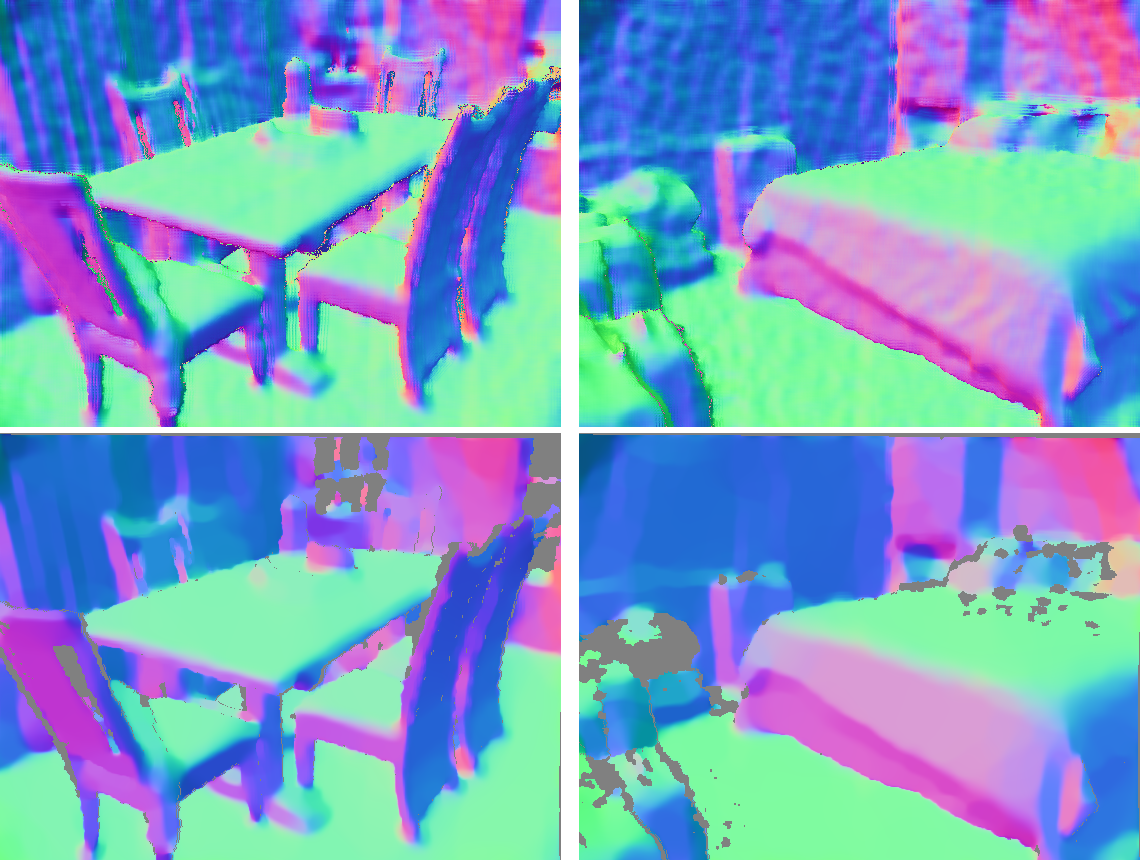
\includegraphics[width=\textwidth]{DenoisedSilberman}
    \caption{Top: normal maps computed based on the method of \citeauthor*{silberman} \cite{silberman} \\ Bottom: masked normal maps after denoising (invalid values are coloured in gray). }
    \label{fig:denoisedsilberman}
\end{figure}

\section{Implementation} \label{sec:datasets}

Three different data sets were created for use in this project: 

\begin{itemize}
    \item A main data set based on the RGB images and depth maps of the NYU Depth V.2 \cite{silberman}, and surface normal maps provided by \citeauthor*{ladicky} \cite{ladicky}.
    \item An alternative data set based on the NYU Depth V.2, and surface normal maps computed based on the method of \citeauthor*{silberman} \cite{silberman}
    \item A data set based on the RGB images and depth maps of the SUN RGB-D \cite{sun}, and surface normal maps computed based on the method of \citeauthor*{silberman} \cite{silberman}
\end{itemize}

\pagebreak

MathWorks MATLAB was used for developing the scripts and functions required for creating the data sets of this project. To build the main data set, first the RGB images and raw depth maps were extracted from NYU Depth V.2 data set. The raw depth data was used to create a mask of invalid data points in each sample (i.e. pixels with missing or invalid depth values). Then, the surface normal maps provided by \citeauthor*{ladicky} were loaded and decoded. These normal maps are provided as PNG images. Because, it was not possible to find any information about the encoding used in the process of converting the original normal maps to these images, the histograms of each channel in several samples were manually analysed to develop a decoding function. Finally, the RGB images and corresponding masked normal maps were stored in a MAT file as output.

To create the alternative data set, similar to main data set, the RGB images and the masks of invalid data points were extracted. The surface normal maps were computed and a denoising technique was applied as discussed in section \ref{sec:surfnormmap}. The masked surface normal maps and RGB images were stored in a MAT file as output.

As mentioned before, the SUN RGB-D data set consists of RGB images and refined depth images in PNG format. To explore the effect of using higher quality samples in this project, only the subset of SUN RGB-D data set is used that has corresponding images in NYU Depth V.2 data set. 

A meta-data data set and a toolbox are also provided for loading and manipulation of data. To create the last data set, the full resolution RGB and raw depth images were loaded by using the information provided in meta-data data set. Similar to the data provided by \citeauthor*{ladicky}, a custom encoding was used for storing the original data in PNG format. Surface normal maps were computed based on the raw depth data and denoising applied on the results. Finally, the RGB images and corresponding masked normal maps were stored in a MAT file.

Figure \ref{fig:sunvsnyu} illustrates the difference in quality of samples obtained from different data sets. In general, samples based on the data obtained from SUN RGB-D have less invalid values (coloured in gray) and slightly less noise. 

\begin{figure}
    \centering
    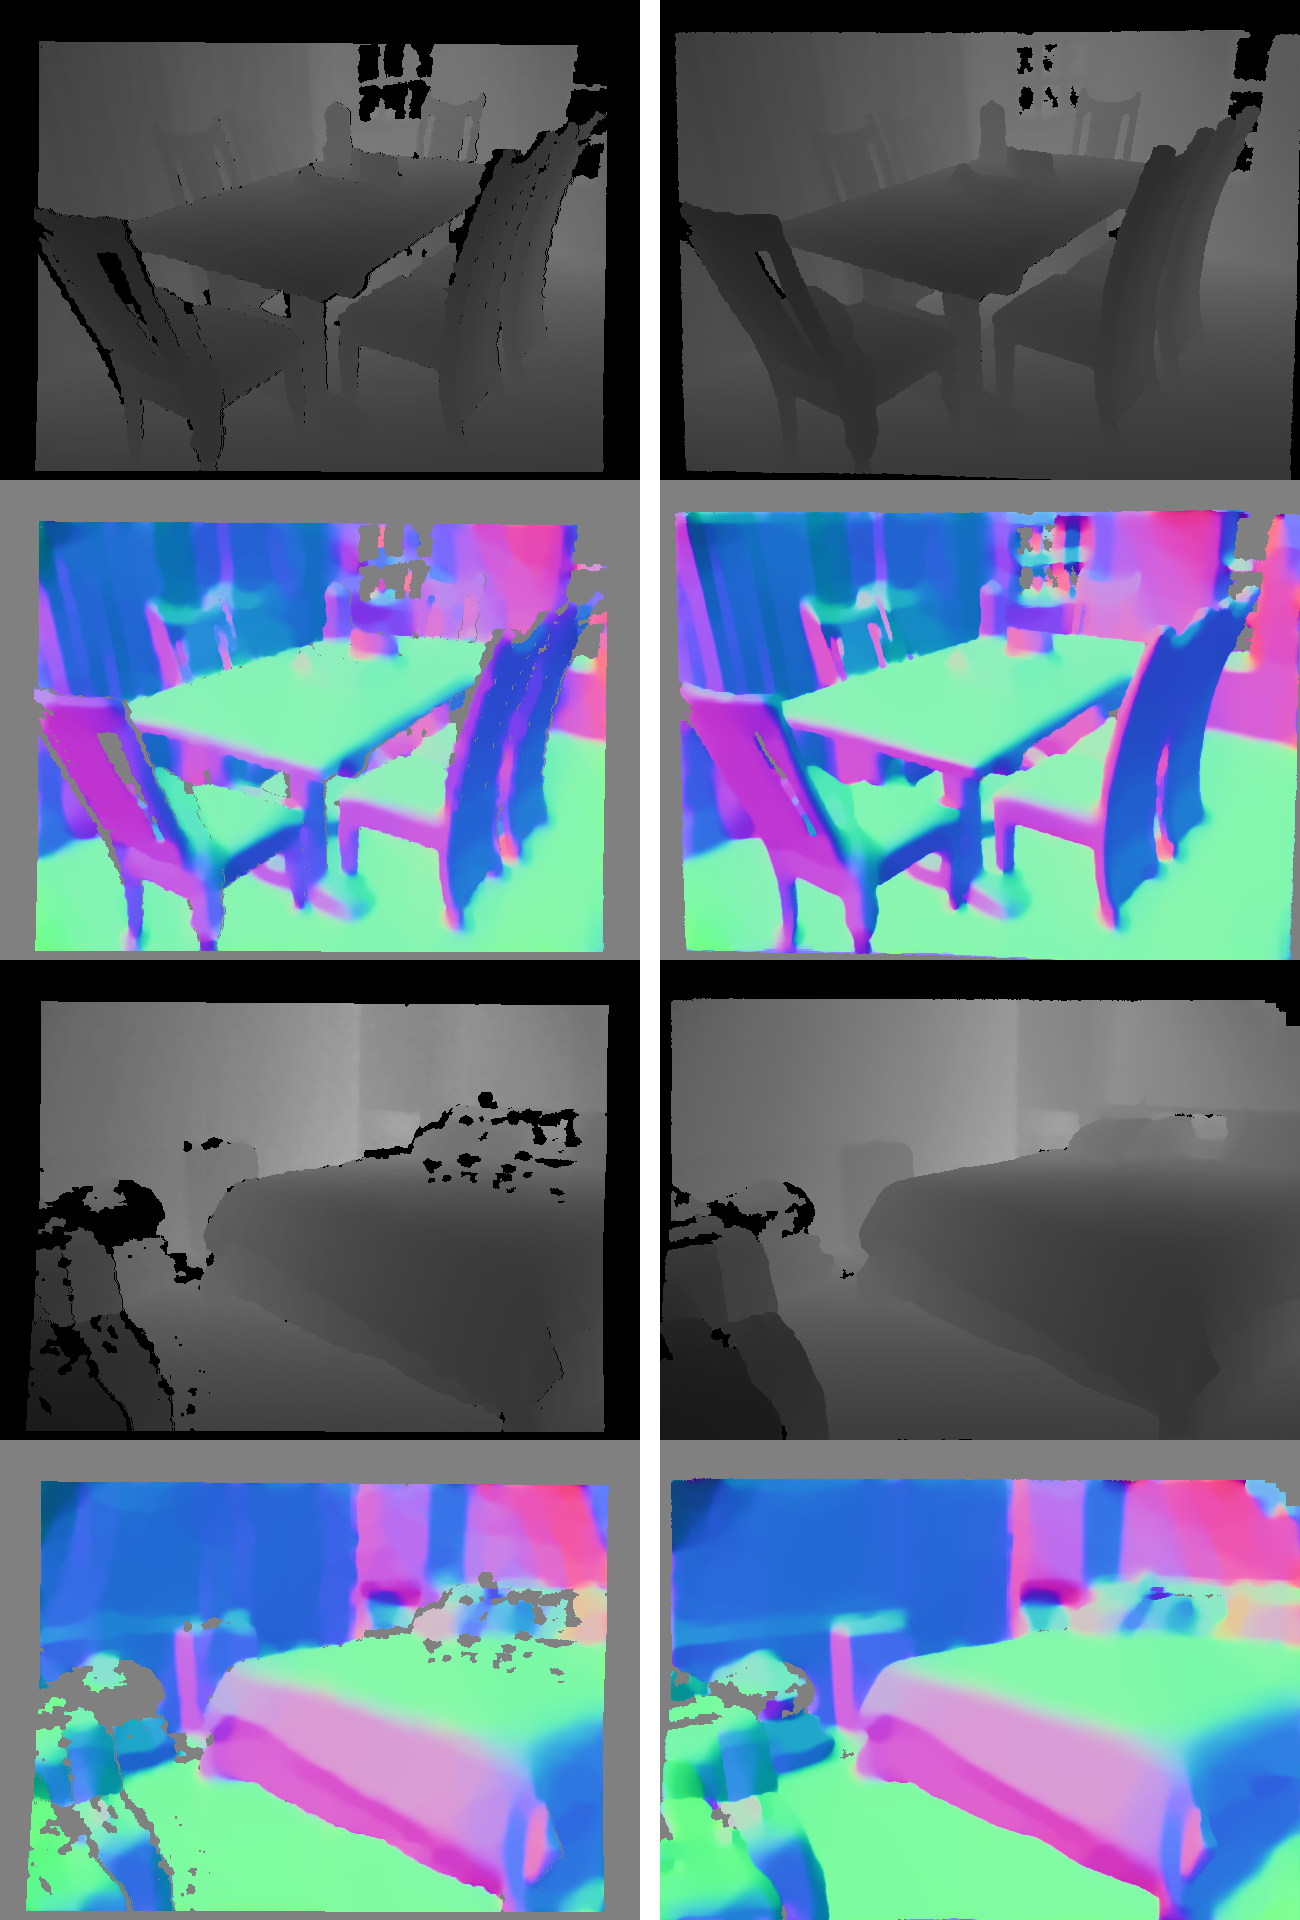
\includegraphics[width=\textwidth]{SUNvsNYU}
    \caption{Left: depth and surface normal maps based on NYU Depth V.2 \\ Right: depth and surface normal maps based on SUN RGB-D}
    \label{fig:sunvsnyu}
\end{figure}

The instructions for obtaining the data sets and source codes are provided in appendix \ref{sec:instructions}. During the development, to ensure the validity and quality of the outputs, code snippets were interactively tested and the output variables were inspected after each modification in their values.



